[6~v\textsuperscript{o}]
Gyri quos dixi continuantur quidem multiplicanturque continuato corporis motu;
sed fracti paulatim atque evanescentes perinde atque ipse corporis motus, ob medii
\edtext{resistentiam\protect\index{Sachverzeichnis}{resistentia medii} et ut ita dicam tenacitatem, quam ab ejus motu oriri credibile est}{\lemma{resistentiam}\Bfootnote{\textit{(1)}\ ab ejus motu ortam \textit{(2)}\ et ut [...] est. \textit{L}}}.
Atque ita corporis motus simul emoritur cum omnibus gyris;
aut si qui restant gyri non sunt sufficientes ad movendum corpus.
\pend
\pstart 
In pleno liquido omnis mutatio difficilis, aestimandaque est tum quantitate mutationis tum liquidi consistentia:
itaque corpus motum sistere, et quietum movere, etiam seclusa gravitate\protect\index{Sachverzeichnis}{gravitas} difficilia.
Motum autem sistere difficilius.
Imo motum sistere et quietum movere sunt inter se, ut linea ad
\edtext{punctum. Pendulorum vibrationes}{\lemma{punctum.}\Bfootnote{\textit{(1)}\ Gyrationes \textit{(2)}\ Pendulorum vibrationes \textit{L}}}
primum valde postea parcius arctantur.
Motus omnes inter se conciliati, ac velut praevisi sunt.
\pend
\count\Bfootins=1200
\pstart
Motus omnes particulares oriuntur a \edtext{generalibus.\\
\hspace*{7,5mm}Omnes conatus manent.}{\lemma{generalibus.}\Bfootnote{\textit{(1)}\ De origi \textit{(2)}\ Omnes [...] manent. \textit{L}}}
\pend
\pstart
Corpus quod sua sponte possit retardato aut accelerato ferri motu, continet mentem.
\pend
\pstart
Corpus \edtext{quod vinculis}{\lemma{quod}\Bfootnote{\textit{(1)}\ sua sponte vi \textit{(2)}\ vinculis \textit{L}}}
quibusdam ad curvam lineam quandam describendam
\edtext{adactum, cessante vinculo}{\lemma{adactum,}\Bfootnote{\textit{(1)}\ si \textit{(2)}\ cessante vinculo \textit{L}}}
continuat motum conatumve in curva, nec movetur per tangentem, id corpus continet mentem.
\pend
\pstart
Ecce discrimen inter impressionem in corporibus et memoriam in mentibus.
\pend
\count\Bfootins=1200
\count\Afootins=1200
\count\Cfootins=1200
\newpage
 \pstart
 \noindent
 \centering
   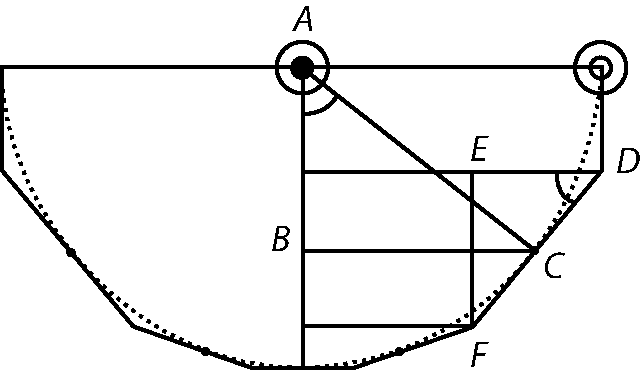
\includegraphics[trim = 0mm -3mm 0mm 0mm, clip, width=0.5\textwidth]{images/lh03705_006v-d1.pdf}\\
    \centering
    [\textit{Fig. 11}]% \caption{\textit{Fig. 11}}
    \pend
    \vspace{1em}
\pstart
$\displaystyle \rule[-4mm]{0mm}{10mm} \frac{DF}{EF} \setline{1}\sqcap \frac{AC}{AB}$.
Jam conatus descendentis in $\displaystyle DF$, est ad conatum descendentis in $\displaystyle EF$,
ut $\displaystyle EF$ ad $\displaystyle DF$, ergo ut $\displaystyle AB$ ad $\displaystyle AC$.
Ergo conatus in \edtext{punctis circumferentiae}{\lemma{punctis}\Bfootnote{\textit{(1)}\ circuli \textit{(2)}\ circumferentiae \textit{L}}}
sunt inter se \edtext{ut sinus complementi}{\lemma{ut}\Bfootnote{\textit{(1)}\ sinus versi \textit{(2)}\  sinus complementi. \textit{L}}}.\\
\hspace*{7.5mm}
\edtext{In descensu gravium\protect\index{Sachverzeichnis}{grave}}{\lemma{In descensu gravium}\Bfootnote{\textit{erg. L}}} Temporibus aequalibus; aequalia sunt celeritatum incrementa\protect\index{Sachverzeichnis}{incrementum celeritatis}.
Ergo celeritates quaesitae sunt ut
\edtext{tempora insumta}{\lemma{tempora}\Bfootnote{\textit{(1)}\ percursa \textit{(2)}\ insumta. \textit{L}}}.
Ergo spatiorum incrementa sunt in ratione temporum.
Ergo spatia ipsa percursa\protect\index{Sachverzeichnis}{spatium percursum} sunt in ratione temporum duplicata,
seu $\displaystyle sa \sqcap t^2$.
Ergo $\displaystyle t \sqcap \sqrt{\vphantom{as}}as$
seu tempora in ratione spatiorum subduplicata.
Ergo si tempora sint ut $\displaystyle AB$,
spatia erunt ut $\displaystyle AC$,
seu descripta parabola $\displaystyle DF$
si tempora sint ut $\displaystyle DG$ vel $\displaystyle EF$,
spatia erunt ut $\displaystyle GF$ vel $\displaystyle DE$.
\pend
%    \vspace{3mm}
%\pstart
%%\vspace{6mm}
%\noindent
%\begin{minipage}[c]{0.5\textwidth}
%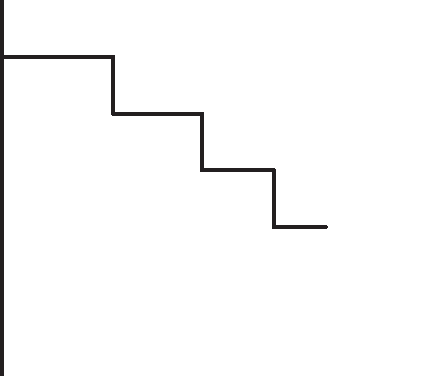
\includegraphics[trim = -30mm -7mm -5mm 0mm, clip, width=0.9\textwidth]{images/lh03705_006v-d2.pdf}
%\end{minipage}
%\hspace*{13,3mm}
%\begin{minipage}[c]{0.5\textwidth}
%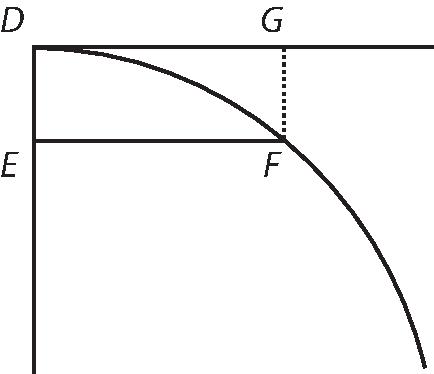
\includegraphics[trim = 0mm -7mm -20mm 0mm, clip, width=0.8\textwidth]{images/lh03705_006v-d3.pdf}
%\end{minipage}
%\hspace*{15mm}
% [\textit{Fig. 12, gestrichen}]\hspace*{50mm} [\textit{Fig. 13}]
%\pend
%\vspace*{2em}
\count\Bfootins=1200
\count\Afootins=1200
\count\Cfootins=1200
\pstart
%\noindent 
Ergo in quolibet spatii puncto temporum crementa erunt in ratione spatiorum
\edtext{percursorum reciproca subduplicata}
{\lemma{percursorum}\Bfootnote{\textit{(1)}\ duplicata \textit{(2)}\ reciproca subduplicata. \textit{L}}}.
Ergo celeritates\protect\index{Sachverzeichnis}{celeritas} sive vires\protect\index{Sachverzeichnis}{vis} erunt in ratione spatiorum percursorum reciproca
\edtext{subduplicata. Ergo quadrata accelerationum erunt inter se in ratione spatiorum}{\lemma{subduplicata.}\Bfootnote{\textit{(1)}\ Et incrementa virium erunt in ratione spatiorum. Ergo si \textit{(a)}\ vires sint inter se in ratione duplicata, erunt \textit{(b)}\ accelerationes in spatiis \textit{(c)}\ spatia sint inter se in ratione \textit{(aa)}\ virium \textit{(bb)}\ numerorum quorundam \textit{(2)}\ Ergo quadrata [...] spatiorum \textit{L}}}
reciproca\edtext{ \edtext{triplicata.\\
\hspace*{7,5mm}Nunc de inclinato impressi conatus sunt in reciproca rectarum}{\lemma{triplicata. [...] rectarum}\Cfootnote{\textit{Zur Variante (1):} \cite{00050}\textsc{G. Galilei}, \textit{Discorsi}, Leiden 1638, S.~166-168 (\cite{00048}\textit{GO} VIII, S.~205-207).}}}{\lemma{triplicata.}\Bfootnote{\textit{(1)}\ Cum celeritates descensu quaesitae \textit{(a)}\ inclinat \textit{(b)}\ ex eadem altitudine inclinato utcunque descensu sint aequales, (videatur Galilaeus\protect\index{Namensregister}{\textso{Galilei (Galilaeus}, Galileus), Galileo 1564-1642|textit}) quoniam scilicet impressi conatus sunt ut spatia, in quolibet momento \textit{(2)}\ Nunc [...] rectarum \textit{L}}}[,] % PR: Hier wurde eine besondere Lösung für die Cfootnote zu einer Bfootnote angewendet.
v.g. $\displaystyle HA$, $\displaystyle BA$.
Ergo et summae eorum seu vires eodem tempore quaesitae.
Ergo et spatiorum crementa; ergo
et spatia percursa iisdem temporibus.
Ergo ponatur recta $\displaystyle AB$ esse $\displaystyle b$,
recta $\displaystyle AH$ esse $\displaystyle h$,
spatium percursum in recta $\displaystyle AH$ esse $\displaystyle y$
et percursum in recta $\displaystyle AB$,
eodem tempore esse $\displaystyle x$,
erit $\displaystyle \rule[-4mm]{0mm}{10mm} \frac{x}{y} \sqcap \rule[-4mm]{0mm}{10mm} \frac{h}{b}$.
seu $\displaystyle x \sqcap \rule[-4mm]{0mm}{10mm} \frac{h}{b} y$.
seu $\displaystyle y \sqcap \rule[-4mm]{0mm}{10mm} \frac{b}{h} x$.
Quod si jam velimus $\displaystyle y$ et $\displaystyle x$ repraesentare in lineis,
et ponamus $\displaystyle AB \sqcap b \sqcap x$.
fiet $\displaystyle y \sqcap \rule[-4mm]{0mm}{10mm} \frac{x^2}{h}$.
Datur $\displaystyle x$, ergo datur et
 [$\displaystyle AC$]\edtext{}{\Bfootnote{$\displaystyle AC \ \sqcap$ \textit{\ L \"{a}ndert Hrsg.}}}.
Jam $\displaystyle AB \, \sqcap \, \sqrt{2aAC}$.
Ergo 
$\displaystyle AC \, \sqcap \, \rule[-4mm]{0mm}{10mm} \frac{AB^2}{2a}$.
seu \edtext{$\displaystyle AC \, \sqcap \frac{x^2}{2a}$.
Quaeratur jam valor ipsius $\displaystyle A(B)$. $\displaystyle \frac{A(B)}{AB} \, \sqcap \, \sqrt{\protect\vphantom{\frac{A(C)}{AC}}}\! \frac{A(C)}{AC} \, \sqcap \, \sqrt{\protect\vphantom{\frac{A(B)}{AH \sqcap h}}}\!\! \frac{A(B)}{AH \sqcap h}$}{\lemma{$\displaystyle AC \, \sqcap \, \frac{x^2}{2a}$.}\Bfootnote{ \textit{ (1) }\ $\displaystyle A(B) \, \sqcap \, \sqrt{2aA(C)}$ et $\displaystyle \frac{A(B)}{h}$ \textit{ (2) }\ Quaeratur [...] $\sqrt{\displaystyle\protect\vphantom{\displaystyle\frac{A(B)}{AH \sqcap \, h}}}\!\! \displaystyle\frac{A(B)}{AH \, \sqcap \, h}$. \textit{ L}}}.
Ergo $\displaystyle \rule[-4mm]{0mm}{10mm} \frac{A(B)^2}{AB^2 \sqcap x^2} \,  \sqcap \,  \frac{A(B)}{h}$.
Ergo $\displaystyle \rule[-4mm]{0mm}{10mm} \frac{A(B)^2}{AB^2 \sqcap x^2} \,  \sqcap \, \frac{A(B)}{h}$.
   Sequitur ergo lineam quae repraesentet $\displaystyle y$
(posito $\displaystyle AB$ esse $\displaystyle x$,)
esse ipsam [$\displaystyle A(B)$]\edtext{}{\Bfootnote{$\displaystyle AB$ \textit{\ L \"{a}ndert Hrsg.}}}.
Quod est id quod invenit
\edtext{Galilaeus\protect\index{Namensregister}{\textso{Galilei} (Galilaeus, Galileus), Galileo 1564-1642}}{\lemma{Galilaeus}\Cfootnote{\cite{00050}a.a.O., S. 95f. und 231f.\cite{00050} (\textit{GO} VIII, S. 139 und 263f.\cite{00048}).}}
nempe per quamlibet circuli chordam eodem tempore
\edtext{ad $\displaystyle A$}{\lemma{ad}\Bfootnote{ \textit{ (1) }\ planum \textit{ (2) }\ $\displaystyle A$ \textit{ L}}} veniri.
\pend
\vspace{3em}
\pstart
%\vspace{6mm}
\noindent
\begin{minipage}[c]{0.5\textwidth}
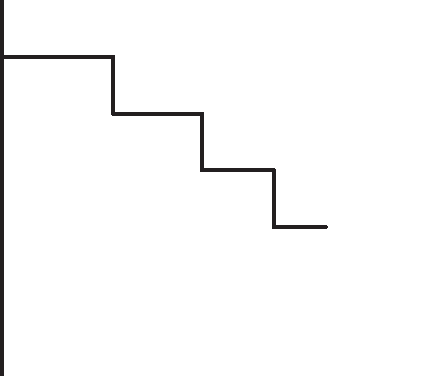
\includegraphics[trim = -30mm -7mm -5mm 0mm, clip, width=0.9\textwidth]{images/lh03705_006v-d2.pdf}
\end{minipage}
\hspace*{13,3mm}
\begin{minipage}[c]{0.5\textwidth}
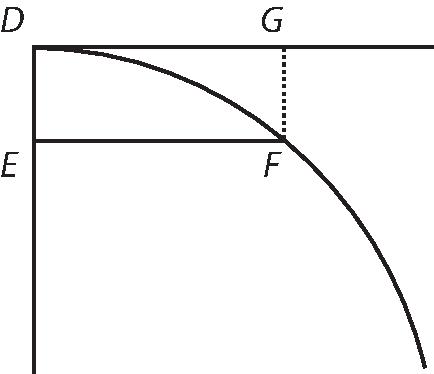
\includegraphics[trim = 0mm -7mm -20mm 0mm, clip, width=0.8\textwidth]{images/lh03705_006v-d3.pdf}
\end{minipage}
\pend
\vspace{0.3em}
\pstart
\hspace*{15mm}
 [\textit{Fig. 12, gestrichen}]\hspace*{50mm} [\textit{Fig. 13}]
\pend
\pstart
\noindent
\centering
 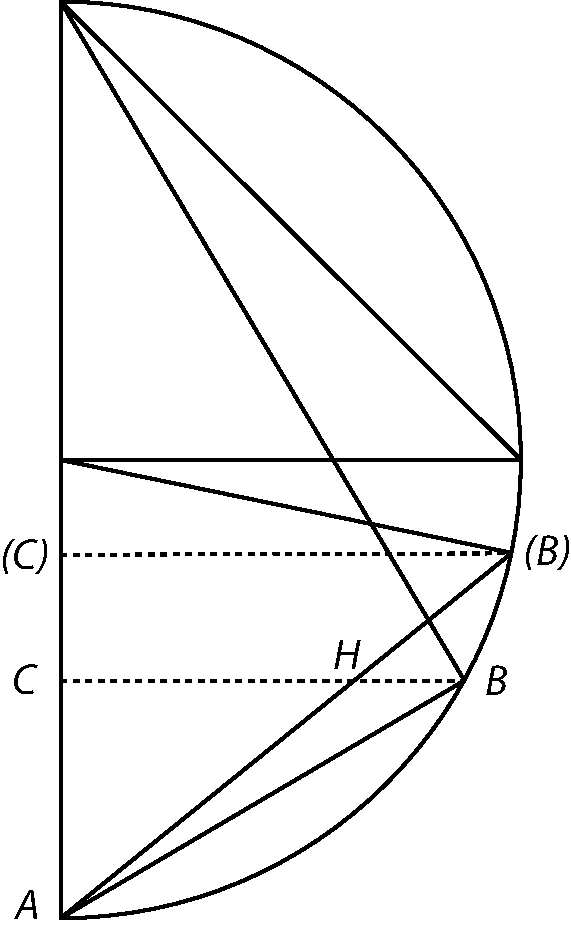
\includegraphics[trim = 0mm -4mm -5mm -6mm, clip, width=0.38\textwidth]{images/lh03705_006v-d4.pdf}\\
    \centering
    [\textit{Fig. 14}]% \caption{\textit{Fig. 14}}
    \pend
\count\Bfootins=1500
\count\Afootins=1500
\count\Cfootins=1500
% PR: Ende des Stückes R/3 